\documentclass[10pt,twoside,twocolumn,openany,nodeprecatedcode]{dndbook}

\usepackage[english]{babel}
\usepackage[utf8]{inputenc}
\usepackage{float, wrapfig, lipsum}

\begin{document}
    \section*{Pact of the Deck}
    At 3rd level, your otherworldly patron bestows upon you a deck of Tarot cards.
    These cards, imbued with the spirits of past holders, grant powers of guidance.
    
    After a long rest, separate the Major and Minor arcana into two decks. From the Major arcana,
    draw a single card. Until your next long rest, this card grants you an ability corresponding to the card.
    See \emph{Major Arcana} for the effects.

    Once per short rest, you may expend a spell slot to redraw your card.

    \section*{Major Arcana}
    \subsection*{0. The Fool}

    \begin{wrapfigure}{l}{0.35\linewidth}
        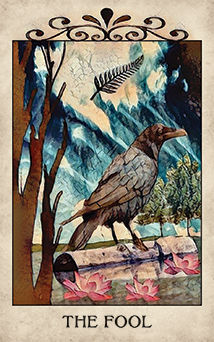
\includegraphics[height=5cm,width=\linewidth]{fool.jpg}
    \end{wrapfigure}
    The Fool is the first card in a Tarot deck because he is the most vulnerable of all the Tarot's archetypes. He has not yet experienced the ups and downs of life, leaving him unaware of the magnitude of life's challenges, and the strength and potential he holds. When The Fool comes up in a Tarot reading, you are encouraged to take on his open, willing energy and embrace all that lies ahead of you without worry.

    \subsubsection*{Ability Granted}
    You can cast \emph{Feather Fall} without expending a spell slot once per short rest.

    \subsection*{1. The Magician}

    \begin{wrapfigure}{l}{0.35\linewidth}
        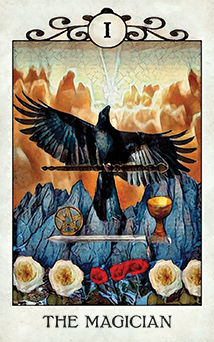
\includegraphics[height=5cm,width=\linewidth]{magician.jpg}
    \end{wrapfigure}
    The Magician card is a reminder that you are a unique being, and have many gifts that others do not hold. These skills set you apart from the crowd, and can help you begin new projects or overcome adversity. When The Magician comes up in your Tarot reading, it's a reminder that you needn't wait -- you already hold everything you need to move forward and accomplish what you've set out to do.

    \subsubsection*{Ability Granted}
    You learn a wizard cantrip of your choice. You are doubly proficient in Arcana.

    \subsection*{2. The High Priestess}

    \begin{wrapfigure}{l}{0.35\linewidth}
        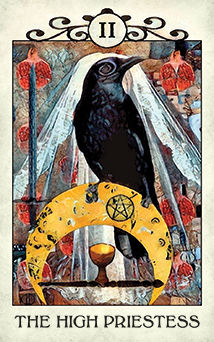
\includegraphics[height=5cm,width=\linewidth]{highpriestess.jpg}
    \end{wrapfigure}
    The most intuitive, connected card in the whole Tarot deck, The High Priestess is a card of awareness and subconsciousness. This card urges you to listen to your inner voice and to follow your instincts. Your mind knows far, far more than you think it does, and The High Priestess embodies this concept. When she arises in your Tarot reading, stop looking for answers in the outside world and instead, turn within for the guidance you seek.

    \subsubsection*{Ability Granted}
    You can cast \emph{Augury} without expending a spell slot once per short rest.

    \subsection*{3. The Empress}

    \begin{wrapfigure}[9]{l}{0.35\linewidth}
        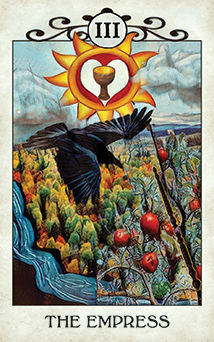
\includegraphics[height=5cm,width=\linewidth]{empress.jpg}
    \end{wrapfigure}
    The Empress is the most feminine card in the Tarot, and she is deeply connected to Mother Nature. When she arises in her deck, she urges you to appreciate, absorb, and utilize the natural world around you.
    \vspace*{50pt}
    \subsubsection*{Ability Granted}
    You can cast \emph{Speak with Animals} without expending a spell slot once per short rest.

    \subsection*{4. The Emperor}

    \begin{wrapfigure}[12]{l}{0.35\linewidth}
        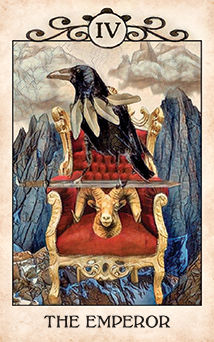
\includegraphics[height=5cm,width=\linewidth]{emperor.jpg}
    \end{wrapfigure}
    The Emperor is a card of leadership and power. He is an authoritative force who has been through many experiences to achieve this status. He represents structure and solidity, and reminds you that you, too, hold immense amounts of power over your own life, and what happens to it.
    \vspace*{10pt}

    \subsubsection*{Ability Granted}
    You are doubly proficient in initimidation. You can cast \emph{command} without expending a spell slot once per short rest.

    \subsection*{5. The Hierophant}

    \begin{wrapfigure}{l}{0.35\linewidth}
        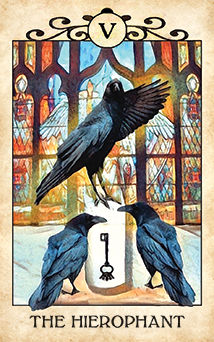
\includegraphics[height=5cm,width=\linewidth]{hierophant.jpg}
    \end{wrapfigure}
    The Hierophant is like a messenger from the heavens. He is experienced in spirituality and guidance, and his job is to bring these lessons down to us here in the real world. When The Hierophant comes up in your Tarot reading, you're encouraged to follow the rules, and to find a spiritual perspective on your current situation.

    \subsubsection*{Ability Granted}
    You can \emph{Turn Undead} once per short rest.

    \subsection*{6. The Lovers}

    \begin{wrapfigure}{l}{0.35\linewidth}
        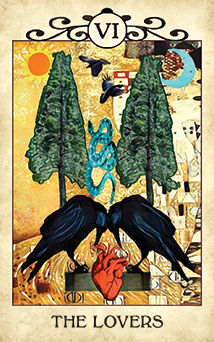
\includegraphics[height=5cm,width=\linewidth]{lovers.jpg}
    \end{wrapfigure}
    It's no surprise The Lovers card represents the close relationships in your life. If it comes up in your Tarot reading, your love life is in need of extra focus and attention. However, this is just as much a card about your values and decisions. You may find The Lovers come up when you are at a crossroads, and must consider all the possible consequences of your choices.

    \subsubsection*{Ability Granted}
    You can cast \emph{Charm Person} once per short rest.

    \subsection*{7. The Chariot}

    \begin{wrapfigure}[12]{l}{0.35\linewidth}
        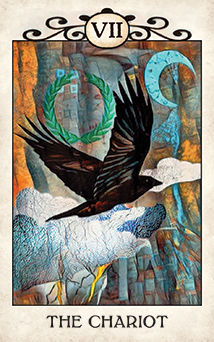
\includegraphics[height=5cm,width=\linewidth]{chariot.jpg}
    \end{wrapfigure}
    The Chariot card is connected to your natural drive and determination, and can indicate an upcoming victory. This card reminds you that your greatest successes won't come through limited thinking -- when you combine the knowledge of your mind with that of your heart \newpage and spirit, you are an unstoppable force.

    \subsubsection*{Ability Granted}
    You and your allies add 15 to their movement speed.

    \subsection*{8. Strength}

    \begin{wrapfigure}{l}{0.35\linewidth}
        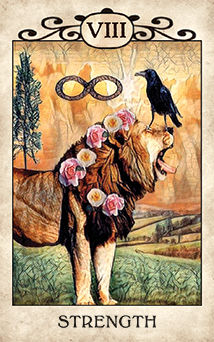
\includegraphics[height=5cm,width=\linewidth]{strength.jpg}
    \end{wrapfigure}
    One of the most obviously named cards in a Tarot deck, Strength is most definitely a card about strength -- but not physical strength. The Strength card represents the fortitude of your heart, your level of courage, and your ability to withstand anything life hands you. If this card arises in your Tarot reading, you are reminded that you are strong enough to handle whatever you are facing -- and will come out of it with even more power than you had before.
    
    \subsubsection*{Ability Granted}
    You are proficient in all saving throws.

    \subsection*{9. The Hermit}

    \begin{wrapfigure}[12]{l}{0.35\linewidth}
        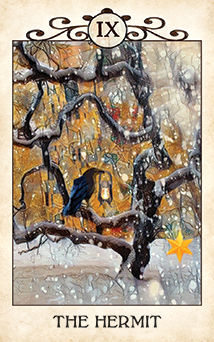
\includegraphics[height=5cm,width=\linewidth]{hermit.jpg}
    \end{wrapfigure}
    The Hermit yearns to be alone. He knows that the only way to process what is happening in life is to withdraw from the noise of the world and create a quiet space of solitude. When The Hermit comes up in your reading, the answers you need will come from within. Be very still, and listen...
    \vspace*{10pt}
    \subsubsection*{Ability Granted}
    You are doubly proficient in insight.

    \newpage

    \subsection*{10. Wheel of Fortune}

    \begin{wrapfigure}[11]{l}{0.35\linewidth}
        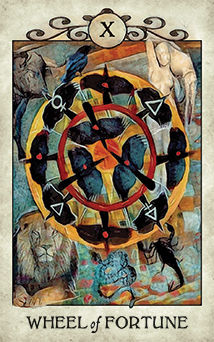
\includegraphics[height=5cm,width=\linewidth]{wheeloffortune.jpg}
    \end{wrapfigure}
    The Wheel of Fortune is constantly revolving -- sometimes you will be at the top, and sometimes you will be at the bottom. This Tarot card reminds you that nothing is permanent, and, good or bad, you must cherish the lessons that this moment is bringing you. 
    \vspace*{30pt}
    \subsubsection*{Ability Granted}
    Instead of rolling, you can declare a result of 20. Your next three rolls are considered 1.

    \subsection*{11. Justice}

    \begin{wrapfigure}{l}{0.35\linewidth}
        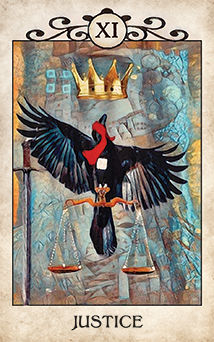
\includegraphics[height=5cm,width=\linewidth]{justice.jpg}
    \end{wrapfigure}
    Justice is your firm-but-fair reminder that karma is real, and there is a consequence for every action. Whatever life is handing you at this moment comes from decisions you've made in the past, and whether it's a punishment or a reward, it is exactly what you deserve. When this card comes up in your Tarot reading, make sure you are acting fairly in all your interactions with others.

    \subsubsection*{Ability Granted}
    Your patron decides whether you have been upholding your pact. If so, +2 AC. If not, your patron can decide to make any one of your rolls a 1 until your next long rest.

    \subsection*{12. The Hanged Man}

    \begin{wrapfigure}[13]{l}{0.35\linewidth}
        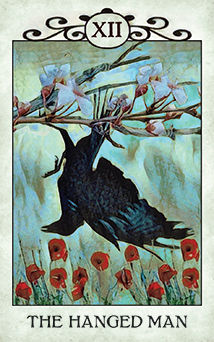
\includegraphics[height=5cm,width=\linewidth]{hangedman.jpg}
    \end{wrapfigure}
    The Hanged Man is a card that comes up when you are in limbo. He tells you that sometimes small sacrifices must be made in order to benefit the bigger picture. When The Hanged Man arises in your reading, you likely want to make a move, but don't even know where to begin. Begin by letting go. Lightening your grip on something that's no longer working for you or detaching from the outcome of your situation can help you release yourself. 

    \subsubsection*{Ability Granted}
    You have no need to breathe, eat, or drink.

    \subsection*{13. Death}

    \begin{wrapfigure}{l}{0.35\linewidth}
        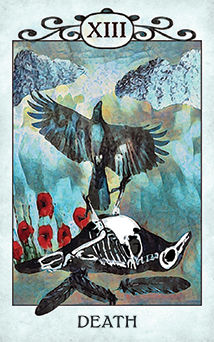
\includegraphics[height=5cm,width=\linewidth]{death.jpg}
    \end{wrapfigure}
    One of the most misunderstood cards in a Tarot deck, Death is not a card about physical death. The Death card speaks of cycles -- endings, yes, but beginnings too -- and is a reminder that all things must pass. Hanging on to relationships, feelings, fears, or situations from the past will hinder you from allowing new, better things to enter your life. Take comfort in knowing that in every ending lies a chance for a new beginning.

    \subsubsection*{Ability Granted}
    You can cast \emph{Speak with Dead} by expending a warlock spell slot.

    \subsection*{14. Temperance}

    \begin{wrapfigure}{l}{0.35\linewidth}
        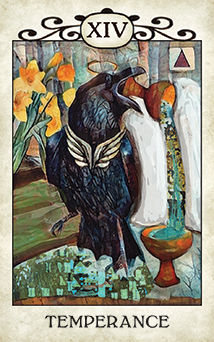
\includegraphics[height=5cm,width=\linewidth]{temperance.jpg}
    \end{wrapfigure}
    The Temperance card is a master of moderation. She encourages peace and patience, and reminds you to go with the flow of your life instead of trying to force its pace or direction. When Temperance turns up in your Tarot reading, it is a message to take things as they come, and remain flexible enough to change with the changes.

    \subsubsection*{Ability Granted}
    You have advantage on saving throws against \emph{illusion} magic.

    \newpage

    \subsection*{15. The Devil}

    \begin{wrapfigure}{l}{0.35\linewidth}
        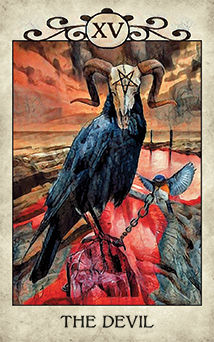
\includegraphics[height=5cm,width=\linewidth]{devil.jpg}
    \end{wrapfigure}
    The Devil card carries heavy feelings of restraint and powerlessness. When he comes up in your Tarot reading, you are likely feeling like you have no control and are stuck in a situation you don't want to be in. The Devil has convinced you that you have no options, but this couldn't be further from the truth. You are not being trapped by external forces, but by your own limitations or unwillingness to move forward. You hold the keys to your own freedom, but it's up to you to open the lock.

    \subsubsection*{Ability Granted}
    Until your next long rest, you become the target of a curse with the effects of \emph{bane}.

    \subsection*{16. The Tower}

    \begin{wrapfigure}{l}{0.35\linewidth}
        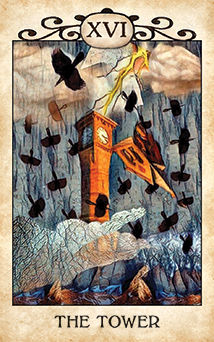
\includegraphics[height=5cm,width=\linewidth]{tower.jpg}
    \end{wrapfigure}
    Perhaps the most dreaded card in a Tarot deck, The Tower is a representation of destruction. The Tower often comes up when everything in your life feels like its crumbling, and you have no way of stopping it. The message of this card is to just let it fall. The weakest parts of your life must be torn down in order to build something strong and sturdy in their place -- something that can last a lifetime.

    \subsubsection*{Ability Granted}
    You lose your deck until you finish your next long rest. 

    \newpage

    \subsection*{17. The Star}

    \begin{wrapfigure}{l}{0.35\linewidth}
        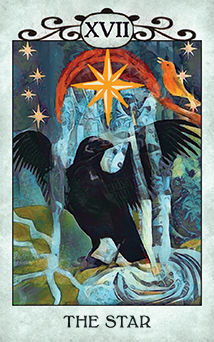
\includegraphics[height=5cm,width=\linewidth]{star.jpg}
    \end{wrapfigure}
    The Star is the embodiment of hope and healing. She is a calming influence that brings messages of renewal, optimism, and inspiration. When The Star comes up in your Tarot reading, she reminds you that the universe is working in your favor, and encourages you to have faith in where you are being taken.

    \subsubsection*{Ability Granted}
    You can cast \emph{faerie fire} without expending a spell slot once per short rest.

    \subsection*{18. The Moon}

    \begin{wrapfigure}{l}{0.35\linewidth}
        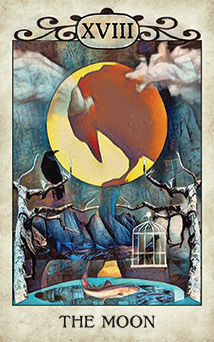
\includegraphics[height=5cm,width=\linewidth]{moon.jpg}
    \end{wrapfigure}
    The Moon card is greatly connected to your subconscious. It represents the thoughts, feelings, doubts and fears that you carry internally. When The Moon arises in your Tarot reading, you may be feeling anxious, allowing these fears to override the memories of your past and your faith in the future. Do not be deceived -- you can't believe everything that you see, hear ... or think. If you can draw these feelings to the surface and address them, you can rid yourself of worry.

    \subsubsection*{Ability Granted}
    You can cast \emph{Disguise Self} without expending a spell slot once per short rest. You are doubly proficient in deception.

    \newpage

    \subsection*{19. The Sun}

    \begin{wrapfigure}{l}{0.35\linewidth}
        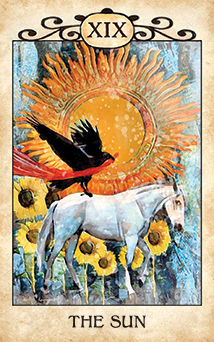
\includegraphics[height=5cm,width=\linewidth]{sun.jpg}
    \end{wrapfigure}
    The Sun is a powerfully uplifting card, representing happiness, joy, vitality, and optimism. When The Sun comes up in your Tarot reading, it is an positive sign that things are working well for you and that you're moving in the right direction. Lift your head and realize all the good situations and people that are surrounding you now and always. 

    \subsubsection*{Ability Granted}
    You can cast \emph{Prayer of Healing} by expending a warlock spell slot.

    \subsection*{20. Judgment}

    \begin{wrapfigure}{l}{0.35\linewidth}
        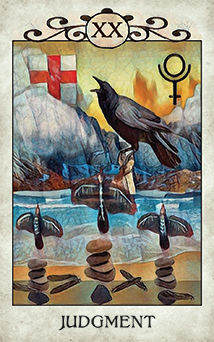
\includegraphics[height=5cm,width=\linewidth]{judgment.jpg}
    \end{wrapfigure}
    Judgment is a card where your past and your future come together. You are being called on to review your decisions and your actions until now, to ensure they are in-line with where you ultimately want to go. The Judgment card reminds you that your future is not set in stone, and that it's never too late to make a change for the better. 

    \subsubsection*{Ability Granted}
    You can cast \emph{detect good and evil} without expending a spell slot once per short rest.

    \subsection*{21. The World}

    \begin{wrapfigure}{l}{0.35\linewidth}
        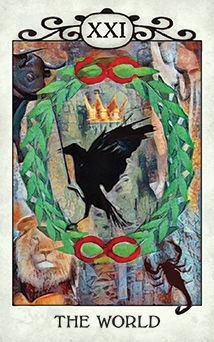
\includegraphics[height=5cm,width=\linewidth]{world.jpg}
    \end{wrapfigure}
    The World is the last card of the Major Arcana, and represents completion, success, and fulfillment. When she arises in your Tarot Reading, The World shows you that you are exactly where you are meant to be on your path. You have a greater understanding of who you are after all you've been through, and you're ready for the next phase of your journey.

    \subsubsection*{Ability Granted}
    Until your next long rest, you can choose to expend this card to be granted the effects of a short rest.


    \section*{Eldritch Invocations}
    \DndFeatHeader{Eldritch Gambit}[Prerequisite: Pact of the Deck]
    You learn the following cantrip. It doesn't count towards your number of cantrips known.

    \DndSpellHeader%
        {Eldritch Gambit}
        {cantrip evocation}
        {1 action}
        {120 feet}
        {V, S}
        {Instantaneous}
    You make a ranged spell attack against a \emph{creature} using the top card of your tarot deck dealing force damage equal to the value of the card.
    The suit of the card determines one of these extra effects:
    \begin{itemize}
        \item Wands: You gain 2 temporary hit point.
        \item Cups: An ally you can see within 120 feet gains 2 temporary hit points.
        \item Swords: Creature hit takes an additional 1d4 damage with the type of your choosing.
        \item Pentacles: 1d4 gold falls to the ground.
    \end{itemize}

    You throw more cards when you reach higher levels: two cards at 5th Level, 
    three cards at 11th level, and four cards at 17th level. 
    You can direct the cards at the same target or at different ones. 
    Make a separate Attack roll for each beam.

\end{document}